\section{Integrated Gradients}\label{section:ig}

Integrated Gradients (IG) \cite{sundararajan2017axiomatic} is a method proposed by Sundararajan et al. that bases on two axioms: \textit{Sensitivity} and \textit{Implementation Invariance}. Authors argue that those two axioms should be satisfied by all attribution methods. The definition of those two axioms is as follows:

\begin{definition}[Axiom: Sensitivity]\label{axiom:sensitivity}
An attribution method satisfies \textit{Sensitivity} if for every input and baseline that differ in one feature but have different predictions, then the differing feature should be given a non-zero attribution. If the function implemented by the deep network does not depend (mathematically) on some variable, then the attribution to that variable is always zero.
\end{definition}

\begin{definition}[Axiom:  Implementation Invariance]\label{axiom:implementation-invariance}
Two networks are functionally equivalent if their outputs are equal for all inputs, despite having very different implementations. Attribution methods should satisfy Implementation Invariance, i.e., the attributions are always identical for two functionally equivalent networks.
\end{definition}

The sensitivity axiom introduces the \textit{baseline} which is an important part of the IG method. Baseline is defined as an \textit{absence of feature} in an input. This definition is confusing, especially when dealing with complex models, but the baseline could be interpreted as \textit{"input from the input space that produces a neutral prediction"}. A baseline can be treated as an input to produce a counterfactual explanation by checking how the model behaves when moving from baseline to the original image.

\begin{remark}
The authors give the example of the baseline for an object recognition network, which is a black image. I personally think that a black image doesn't represent an "absence of feature", because this absence should be defined based on the manifold that represents data. This means that a black image could work as an absence of a feature in one network but may not work for a network trained on a different dataset, allowing a network to use black pixels in prediction.
\end{remark}


\begin{wrapfigure}{R}{0.30\textwidth}
  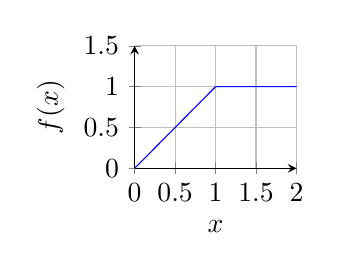
\begin{tikzpicture}
    \begin{axis}[
        axis lines = left,
        xlabel = $x$,
        ylabel = {$f(x)$},
        width=0.3\textwidth,
        ymax = 1.5,
        grid=both,
        legend pos=north east,
    ]
    %Here the blue parabloa is defined
    \addplot [
        domain=0:2, 
        samples=100, 
        color=blue,
        ]
        {1 - max(0, 1- x)};
    
    \end{axis}
    \end{tikzpicture}
  \caption{Values of $f(x) = 1 - \text{ReLU}(1 - x)$ where $x \in <0,2>$}\label{fig:ig-relu-example}
\end{wrapfigure}

Authors argue that gradient-based methods are violating Sensitivity (Def. \ref{axiom:sensitivity}). As an example, we are presented with the case of simple function, $f(x) = 1 - \text{ReLU}(1 - x)$ (see Fig. \ref{fig:ig-relu-example}) and the baseline being $x = 0$. When trying to generate attribution for $x = 2$, the functions' output changes from 0 to 1 but after $x=1$, it becomes flat and causes the gradient to equal zero. Obviously, $x$ attributes to the result, but because the function is flat at the input we are testing results in invalid attribution and breaks the Sensitivity. Sundararajan et al. think that breaking Sensitivity causes gradients to focus on irrelevant features.

\vspace{\baselineskip}

In IG definition we have a function $F$ representing our model, input $x \in \mathbb{R}^{n}$ ($x$ is in $\mathbb{R}^n$ because this is a general definition of IG and not CNN specific), and the baseline $x' \in \mathbb{R}^{n}$. We assume straightline path between $x$ and $x'$ and compute gradients long that path. The integrated gradient along $i^th$ dimension is defined as:

\begin{equation}
    IntegratedGrads_{i}(x) ::= (x_{i} - x'_{i})\times\int_{\alpha=0}^1\frac{\partial F(x'+\alpha \times (x - x'))}{\partial x_i}{d\alpha}
    \label{eq:ig-full-eq}
\end{equation}

The original definition of Integrated Gradients is incalculable (because of integral). Therefore, the implementation of the method uses approximated value by replacing the integral with summation:

\begin{equation}
    IntegratedGrads^{approx}_{i}(x)::=(x_{i}-x'_{i})\times\sum_{k=1}^{m}\frac{\partial F(x' + \frac{k}{m}\times(x - x'))}{\partial x_{i} } \times \frac{1}{m}
    \label{eq:ig-aprox}
\end{equation}

In the approximated calculation (Eq. \ref{eq:ig-aprox}), $m$ defines a number of interpolation steps. As an example, we can visualize the interpolations with $m$ equals five (see Fig. \ref{fig:ig-interpolation}). In practice, the number of interpolation steps is usually between 20 and 300, but the mode value is equal to 50. The results of applying IG can be seen in Figure \ref{fig:ig-saliency-map-bernard}.

\begin{figure}[ht]
    \centering
    \includegraphics[width=\textwidth]{methods/images/ig-saint_bernard-interpolation.png}
 \caption{Five-step interpolation between the baseline $x'$ and the input image $x$. The first image on the left ($\text{alpha:} 0.0$) is not a part of the interpolation process. Image source: \textit{Stanford Dogs} \cite{stanford-dogs} }\label{fig:ig-interpolation}
\end{figure}

\begin{wrapfigure}{L}{0.30\textwidth}
  \includegraphics[width=0.30\textwidth]{methods/images/ig-saint_bernard.png}
  \caption{Visualization of the saliency map by the IG generated for the class \textit{saint\_bernard}. The result is averaged over 50 interpolation steps. Image source: \textit{Stanford Dogs} \cite{stanford-dogs}}\label{fig:ig-saliency-map-bernard}
\end{wrapfigure}

In recent years there was discussion about replacing constant color baseline with an alternative. One of the first propositions was to add Gaussian noise to the original image (see Fig. \ref{fig:ig-baseline-gaussian}. \textit{Gaussian baseline} was introduced by Smilkov et al. \cite{smilkov2017smoothgrad} and used a Gaussian distribution centered on the current image with a variance $\sigma$. This variance is the only parameter when tuning the method. Another baseline is called \textit{Blur baseline} and uses a multi-dimensional gaussian filter (see Fig. \ref{fig:ig-baseline-blur}). The idea presented by Fong and Vedaldi \cite{fong2017interpretable} blurred version of the image is a domain-specific way to represent missing information and therefore be a valid baseline according to the original definition. Inspired by the work of Fong and Vedaldi, Sturmfels et al. \cite{sturmfels2020visualizing} introduced another version of the baseline, which is based on the original image. This baseline is called the \textit{Maximum Distance baseline} and creates a baseline by constructing an image with the largest value of the $L1$ distance from the original image. The result of that can be seen in Figure \ref{fig:ig-baseline-max-dist}. The problem with the maximum distance is that it doesn't represent the "absence of feature". It contains the information about the original image, just in a different form. In the same work, Sturmfels et al. created another baseline called \textit{Uniform baseline}. This time, the baseline doesn't require an input image and uses only uniform distribution to generate a baseline (see Fig. \ref{fig:ig-baseline-uniform}). The problem with selecting a baseline is not solved, and for any further experiments, the "black image" baseline is going to be used.


\begin{figure}[h]
  \centering
 \begin{subfigure}{.23\textwidth}
    \centering
    \includegraphics[width=\textwidth]{methods/images/ig-saint_bernard-gaussian.png}
    \caption{Gaussian Baseline}\label{fig:ig-baseline-gaussian}
\end{subfigure}
 \begin{subfigure}{.23\textwidth}
    \centering
    \includegraphics[width=\textwidth]{methods/images/ig-saint_bernard-blur.png}
    \caption{Blur Baseline}\label{fig:ig-baseline-blur}
\end{subfigure}
 \begin{subfigure}{.23\textwidth}
    \centering
    \includegraphics[width=\textwidth]{methods/images/ig-saint_bernard-max-dist.png}
    \caption{Max Distance Baseline}\label{fig:ig-baseline-max-dist}
\end{subfigure}
 \begin{subfigure}{.23\textwidth}
    \centering
    \includegraphics[width=\textwidth]{methods/images/ig-saint_bernard-uniform.png}
    \caption{Uniform Baseline}\label{fig:ig-baseline-uniform}
\end{subfigure}

 \caption{Alternative baselines for IG. Gaussian baseline is using $\sigma = 0.5$ to generate noise. Blur baseline is using $\sigma = 5$ in a gaussian filter. All the values are clipped at $<0,1>$ to be within the range of the scaled colors. Image source: \textit{Stanford Dogs} \cite{stanford-dogs} }\label{fig:ig-alternative baselines}
\end{figure}